\documentclass{beamer}
\mode<presentation> {
  \usetheme{Madrid} % or try Darmstadt, Madrid, Warsaw, ...
  \usecolortheme{default} % or try albatross, beaver, crane, ...
  \usefonttheme{default}  % or try serif, structurebold, ...
  \setbeamertemplate{navigation symbols}{}
  \setbeamertemplate{caption}[numbered]
} 

\usepackage[english]{babel}
\usepackage[utf8x]{inputenc}
\usepackage{graphicx}
\usepackage{amsmath}
\usepackage{amsfonts}
\usepackage{amssymb}
\usepackage{hyperref}

\usepackage{import}
\usepackage{standalone}
\usepackage{wrapfig}

\usepackage{tikz}
\usepackage{subcaption}
\usetikzlibrary{calc}
\usetikzlibrary {shapes.geometric}

%Defines theorem enviroments
\theoremstyle{definition}


\title[The 17 Wallpaper Groups]{Frieze Groups, Lattices and Wallpaper groups}
\author{Braydon Xuereb, James Butcher, Rory Yarr}
\institute[University of Newcastle] % (optional)
{
  MATH3120 Abstract Algebra \\
  University of Newcastle
}
\date{4 June, 2024}

\begin{document}

\begin{frame}
  \titlepage
\end{frame}
\begin{frame}{Wallpaper groups}
    \begin{figure}
        \centering
        \includegraphics[width=0.9\textwidth]{Figures/WallpaperGroupsExample.png}
        \caption{The 17 wallpaper groups \cite{Clark1}}
        \label{fig:17WallpaperGroups}
    \end{figure}
\end{frame}

\begin{frame}
  \frametitle{Introduction, group operations}
  \begin{definition}[Types of Symmetries]
  \begin{itemize}
      \item Translations 
      \item Reflections
      \item Glide Reflections
      \item Rotations.
  \end{itemize}
  \end{definition}
\end{frame}



\begin{frame}{Translations }
\begin{definition}
     Translations are repetitions of a pattern structure.  defined mathematically as follows \\ 
    a mapping $t_a$ : $\mathbb{R}^2 \rightarrow \mathbb{R}^2$ where $x \rightarrow x + a $ where $x \in X$  \cite{Angela:2023}
\end{definition}
   \begin{figure}
        \centering
        
\begin{tikzpicture}
            % Draw glide
            \draw[->] (1.5,0.5) -- (2.5,0.5);
            % Normal text above the line
            \node at (0,0.5) {\huge Pattern};
            % Translated text
            \node at (4,0.5) {\huge Pattern};
        \end{tikzpicture}
        \caption{Translations}
        \label{Reflection}
    \end{figure}
\end{frame}

\begin{frame}{Reflections and Glide reflections}
    \begin{definition}
        Reflections: A reflection over a line through the origin is defined as follows\\
        $Ref_l(v) =$ \(2\frac{v \cdot l}{l \cdot l}\)l - v\\ where v and l are vectors going through the line of origin.\\ 
        Glide : A glide is a reflection followed by a translation.  \cite{Angela:2023}
    \end{definition}
    \begin{figure}
        \centering
        \input{OtherDiagrams/Reflections and Glide Reflections}
        \caption{Reflective Symmetries}
        \label{fig:symmetries}
    \end{figure}
\end{frame}

\begin{frame}{Rotations}
    \begin{definition}
        A rotation is a change of angle around a center point.
        $R_\theta = \begin{bmatrix}
            \cos\theta & -\sin\theta\\
            \sin\theta & \cos\theta
        \end{bmatrix}$ 
        Where $\theta \in \{1,2,3,6\}.$ \cite{Angela:2023}
    \end{definition}
    \begin{figure}
        \centering
        \input{OtherDiagrams/Rotations}
        \caption{Rotations}
        \label{fig:enter-label}
    \end{figure}
\end{frame}

\begin{frame}{Lattices}
    \begin{definition}
        A lattice is the group $(\mathbb{Z}[\Vec{a},\Vec{b}],+).$\\
        i.e., a grid of points where any point $p = n\Vec{a} +m\Vec{b}$ 
    \end{definition}
    \begin{figure}
        \centering
        \scalebox{0.5}{\input{OtherDiagrams/LatticeDiagram}}
        \caption{Lattice}
        \label{fig:enter-label}
    \end{figure}
\end{frame}

\begin{frame}{Bravais Lattices}
    \begin{minipage}{0.35\textwidth}
        Primitive cells are parallelograms, whereas centered cells have lattice points in the center.

        Additionally, Square $\subseteq$ Rectangle $\subseteq$ Rhombic,
        The Rectangle $\subseteq$ Oblique cell and the Hexagonal cell $\subseteq$ Oblique Cell.
    \end{minipage}
    \hfill
    \begin{minipage}{0.6\textwidth}
        \centering
        \scalebox{0.6}{\input{Bravais Lattice Diagrams/Bravais Lattices}}
        \captionof{figure}{Bravais Lattices}
        \label{fig:lattice}
    \end{minipage}
\end{frame}
\begin{frame}{Visual proof that lattices cannot have order 8}
\begin{figure}
    \centering
    \begin{minipage}{0.3\textwidth}
        \scalebox{0.5}{\input{Bravais Lattice Diagrams/Proof1}}
        \caption{1}
    \end{minipage}
    \hfill
    \begin{minipage}{0.3\textwidth}
        \scalebox{0.5}{\input{Bravais Lattice Diagrams/Proof2}}
        \caption{2}
    \end{minipage}
    \hfill
    \begin{minipage}{0.3\textwidth}
        \scalebox{0.5}{\input{Bravais Lattice Diagrams/Proof3}}
        \caption{3}
    \end{minipage}
    \caption{Octagons under translation}
    \label{fig:enter-label}
\end{figure}
    \begin{block}{Proof sketch}
        Note that any point can translated by lattice definition. So the translation of the center and vertices gives two smaller octagons. This can further be extended in smaller octagons. This can be repeated infinitely. Creating a dense grid of points on the entire 2-dimensional plane.
    \end{block}
\end{frame}

\begin{frame}{Frieze Groups}
    \begin{definition}
        A frieze group is the set of two-dimensional patterns that repeat in one dimension. \cite{Ganapathy:2021}
    \end{definition}
    \begin{figure}
        \centering
        \input{OtherDiagrams/FriezeGroupDiagram}
        \caption{Frieze group example}
        \label{fig:enter-label}
    \end{figure}
\end{frame}

\begin{frame}{Frieze Groups}
    \begin{figure}
    \centering
	\input{Figures/Frieze groups/FriezeGroups}
	\caption{The seven frieze groups \cite{Tomruen:2015}.}
	\label{fig:FriezeGroups}
\end{figure}
\end{frame}

\begin{frame}{Wallpaper Groups}
    \begin{definition}
        A wallpaper group is the set of isometries and a fundamental region that fill an entire two-dimensional Euclidean plane. \cite{Ganapathy:2021}
    \end{definition}
    \begin{figure}
        \centering
        \documentclass[class=article, crop=false]{standalone}
\usepackage{tikz}
\usepackage{subcaption}
\usetikzlibrary{calc}

\begin{document}

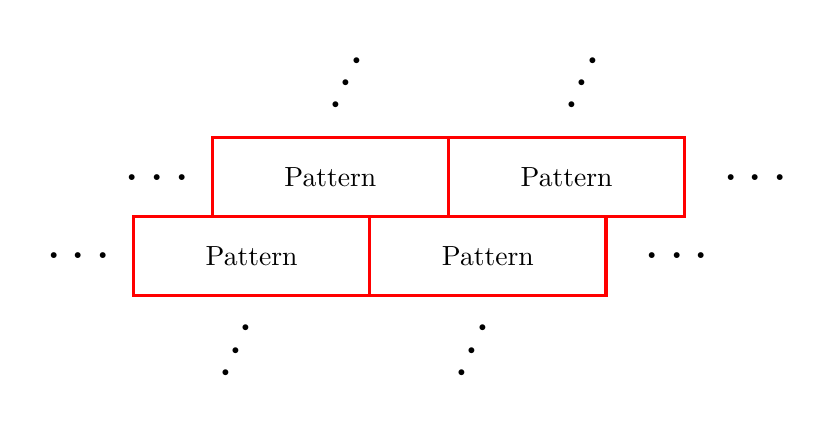
\begin{tikzpicture}
        % Add ellipses at start
        \node[scale=2] at (-0.2, .5) {$\ldots$};
        \node[scale=2] at (0.8, 1.5) {$\ldots$};
        \foreach \i in {0,...,1} {
            \foreach \j in {0,...,1} {
                \draw[red, very thick] (0.5+3*\i+\j,1*\j) rectangle (3.5+3*\i+\j,1*\j+1);
                \node at (2 + 3*\i+\j, 1*\j+.5) {Pattern};
        }}
        % Add ellipses at the end
        \node[scale=2] at (7.4, .5) {$\ldots$};
        \node[scale=2] at (8.4, 1.5) {$\ldots$};
        % Add ellipses above
        \node[scale=2,rotate=-115] at (3.2, 2.7) {$\ldots$};
        \node[scale=2,rotate=-115] at (6.2, 2.7) {$\ldots$};
        % Add ellipses below
        \node[scale=2,rotate=-115] at (1.8, -0.7) {$\ldots$};
        \node[scale=2,rotate=-115] at (4.8, -0.7) {$\ldots$};
    \end{tikzpicture}

\end{document}
        \caption{Wallpaper group example}
        \label{fig:enter-label}
    \end{figure}
\end{frame}

\begin{frame}{Symmetry group properties, IUC}
    \begin{table}
    \begin{tabular}{|c|c|c|c|}
        \hline
        Wallpaper Group & Lattice & Rotation order & Reflections \\
        \hline
        p1 & Oblique & 0 & none\\
        p2 & Oblique & 2 & none\\
        pm & Rectangle & 0 & 180$^\circ$\\
        pg & Rectangle & 0 & none\\
        cm & Rhombus & 0 & 180$^\circ$\\
        pmm & Rectangle & 2 & 90$^\circ$\\
        pmg & Rectangle & 2 & 180$^\circ$\\
        pgg & Rectangle & 2 & none\\
        cmm & Rhombus & 2 & 90$^\circ$\\
        \hline
    \end{tabular}   
    \caption{Symmetries of the wallpaper groups. \cite{Clark1}}
\end{table}
\end{frame}
\begin{frame}{Symmetry group properties, IUC}
    \begin{table}
        \begin{tabular}{|c|c|c|c|}
            \hline
            Wallpaper Group & Lattice & Rotation order & Reflections \\
            \hline
            p4 & Square & 4 & none\\
            p4m & Square & 4$^\dagger$ & 45$^\circ$\\
            p4g & Square & 4$^*$ & 90$^\circ$\\
            p3 & Hexagon & 3 & none\\
            p31m & Hexagon & 3$^*$ & 60$^\circ$\\
            p3m1 & Hexagon & 3$^\dagger$ & 30$^\circ$\\
            p6 & Hexagon & 6 & none\\
            p6m & Hexagon & 6 & 30$^\circ$\\
            \hline
        \end{tabular}
    \caption{Symmetries of the wallpaper groups: $\dagger$ means the rotation centres lie on the reflection axis. * means the group rotation centres are not on the reflection axis. \cite{Clark1}}
\end{table}
\end{frame}

\begin{frame}
\frametitle{Wall Paper Groups}
    \begin{block}{Why are they A group}
        They meet the three group axioms
        \begin{itemize}
            \item Identity: no transformations.
            \item Inverses: the reversal or opposite of the transformation.
            \item Associativity: two transformations are still a transformation. \cite{Angela:2023}
        \end{itemize}       
    \end{block}
\end{frame}

\begin{frame}
  \frametitle{Wallpaper groups}
  \begin{columns}
          \column{0.5\linewidth}
  \begin{definition}
      \begin{itemize}
          \item P1 (primitive of order 1)\cite{Trefor1}
          \item simplest of the 17 groups 
          \item consists only of translations
      \end{itemize}
  \end{definition}/
  \column{0.4\textwidth}
  \includegraphics[width=\textwidth]{Figures/p_examples/eschersketch_p1_example_person.png}
  \end{columns}
  \begin{figure}
        \centering
        \scalebox{0.7}{\input{Wallpaper Group Diagrams/p1}}
        \caption{p1 diagram}
        \label{fig:p1}
  \end{figure}
\end{frame}

\begin{frame}
\frametitle{more examples of wallpaper groups}
    \begin{figure}
     \centering
     \begin{subfigure}[b]{0.3\textwidth}
         \centering
         \includegraphics[width=\textwidth]{Figures/p_examples/p_2_simple.JPG}
         \caption{p2}
         \label{fig: p2}
     \end{subfigure}
     \hfill
     \begin{subfigure}[b]{0.3\textwidth}
         \centering
         \includegraphics[width=\textwidth]{Figures/p_examples/p_3_simple.JPG}
         \caption{p3}
         \label{fig:p3}
     \end{subfigure}
     \vfill
     \begin{subfigure}[b]{0.3\textwidth}
         \centering
         \includegraphics[width=\textwidth]{Figures/p_examples/p_4_simple_two.JPG}
         \caption{p4}
         \label{fig:p4}
     \end{subfigure}
     \hfill
     \begin{subfigure}[b]{0.3\textwidth}
         \centering
         \includegraphics[width=\textwidth]{Figures/p_examples/P6.png}
         \caption{p6}
         \label{fig:p6}
     \end{subfigure}
        \caption{Four of the simplest wallpaper groups}
        \label{fig:The four ps}       
\end{figure}
\end{frame}
    
\begin{frame}{p6m}
    \begin{figure}{\textwidth}
        \centering
        \begin{minipage}{0.6\textwidth}
            \centering
            \begin{subfigure}[b]{\textwidth}
                \centering
                \includegraphics[width=0.5\textwidth]{Figures/p6m/p6m_full.JPG}
                \caption{Image of p6m}
                \label{fig:p6m_full}
            \end{subfigure}
            \vfill
            \begin{subfigure}[b]{\linewidth}
                \centering
                \includegraphics[width=0.5\linewidth]{Figures/p6m/p6m_simplified.png}
                \caption{p6m zoomed into one cell}
                \label{fig:p6m_zoomed}
            \end{subfigure}
        \end{minipage}
        \hspace{-2cm} % Adjust this value to control the space
        \begin{minipage}{0.35\textwidth}
            \begin{subfigure}[b]{\textwidth}
                \centering
                \scalebox{0.55}{\input{Wallpaper Group Diagrams/p6m}}
                \caption{p6m Diagram}
                \label{fig:p6m_diagram}
            \end{subfigure}
        \end{minipage}
        \caption{One of the most complex wallpaper groups}
        \label{fig:The four ps}
    \end{figure}
\end{frame}

\begin{frame}
  \frametitle{Conclusion}
  \begin{itemize}
    \item The 17 Wallpaper groups are a mathematical repetitive 2D pattern.
    \item There are 4 symmetries within each group: translation, rotation, reflection and glide reflection.
    \item The 7 Frieze groups are 2D unidirectional patterns.
    \item There are 5 lattices: square, rectangular, rhombic, oblique, hexagonal. 
    \item Implications or potential applications of the research: art, crystallography, engineering, etc.
  \end{itemize}
\end{frame}
\begin{frame}{Wallpaper generators to play around with if we have time}
\begin{itemize}
    \item  \href{https://singsurf.org/wallpaper/wallpaper.php?FILENAME=101837470_6beae39fe1.jpg}{Image wallpaper Generator}
    \item \href{https://math.hws.edu/eck/js/symmetry/wallpaper.html}{Drawing Wallpaper generator}
\end{itemize}
    
\end{frame}

\begin{frame}{Questions}
  \begin{figure}
    \centering
    % Row 1
    \begin{minipage}{0.16\textwidth}
        \centering
        \scalebox{0.10}{\input{Wallpaper Group Diagrams/p1}}
        \caption*{p1}
    \end{minipage}
    \hfill
    \begin{minipage}{0.14\textwidth}
        \centering
        \scalebox{0.10}{\input{Wallpaper Group Diagrams/p2}}
        \caption*{p2}
    \end{minipage}
    \hfill
    \begin{minipage}{0.10\textwidth}
        \centering
        \scalebox{0.15}{\input{Wallpaper Group Diagrams/pm}}
        \caption*{pm}
    \end{minipage}
    \hfill
    \begin{minipage}{0.10\textwidth}
        \centering
        \scalebox{0.10}{\input{Wallpaper Group Diagrams/pg}}
        \caption*{pg}
    \end{minipage}
    \hfill
    \begin{minipage}{0.15\textwidth}
        \centering
        \scalebox{0.10}{\input{Wallpaper Group Diagrams/cm}}
        \caption*{cm}
    \end{minipage}
    % Row 2
    \vfill
    \begin{minipage}{0.16\textwidth}
        \centering
        \scalebox{0.10}{\input{Wallpaper Group Diagrams/cmm}}
        \caption*{cmm}
    \end{minipage}
    \hfill
    \begin{minipage}{0.10\textwidth}
        \centering
        \scalebox{0.10}{\input{Wallpaper Group Diagrams/pmm}}
        \caption*{pmm}
    \end{minipage}
    \hfill
    \begin{minipage}{0.16\textwidth}
        \centering
        \scalebox{0.15}{\input{Wallpaper Group Diagrams/pmg}}
        \caption*{pmg}
    \end{minipage}
    \hfill
    \begin{minipage}{0.16\textwidth}
        \centering
        \scalebox{0.15}{\input{Wallpaper Group Diagrams/p4}}
        \caption*{p4}
    \end{minipage}
    \vfill
    % Row 3
    \begin{minipage}{0.10\textwidth}
        \centering
        \scalebox{0.10}{\input{Wallpaper Group Diagrams/p4m}}
        \caption*{p4m}
    \end{minipage}
    \hfill
     \begin{minipage}{0.10\textwidth}
        \centering
        \scalebox{0.10}{\input{Wallpaper Group Diagrams/p3}}
        \caption*{p3}
    \end{minipage}
    \hfill
    \begin{minipage}{0.16\textwidth}
        \centering
        \scalebox{0.10}{\input{Wallpaper Group Diagrams/p4g}}
        \caption*{p4g}
    \end{minipage}
    \hfill
    \begin{minipage}{0.10\textwidth}
        \centering
        \scalebox{0.13}{\input{Wallpaper Group Diagrams/pgg}}
        \caption*{pgg}
    \end{minipage}
    % Row 4
    \vfill
    \begin{minipage}{0.10\textwidth}
        \centering
        \scalebox{0.10}{\input{Wallpaper Group Diagrams/p6}}
        \caption*{p6}
    \end{minipage}
    \hfill
    \begin{minipage}{0.16\textwidth}
        \centering
        \scalebox{0.10}{\input{Wallpaper Group Diagrams/p6m}}
        \caption*{p6m}
    \end{minipage}
    \hfill
    \begin{minipage}{0.10\textwidth}
        \centering
        \scalebox{0.10}{\input{Wallpaper Group Diagrams/p3m1}}
        \caption*{p3m1}
    \end{minipage}
    \hfill
    \begin{minipage}{0.10\textwidth}
        \centering
        \scalebox{0.10}{\input{Wallpaper Group Diagrams/p31m}}
        \caption*{p31m}
    \end{minipage}
    \caption{The 17 Wallpaper Groups}
    \label{fig:17-wallpaper-groups}
\end{figure}
\end{frame}

\begin{frame}

  \frametitle{References}
  \bibliographystyle{apalike} % We choose the "plain" reference style
  \bibliography{Sources} % Entries are in the refs.bib file
\end{frame}

\begin{frame}{p1 cell diagram}
    \begin{figure}
        \centering
        \input{Wallpaper Group Diagrams/p1}
        \caption{p1 cell diagram.}
        \label{fig:enter-label}
    \end{figure}
\end{frame}

\begin{frame}{p2 cell diagram}
    \begin{figure}
        \centering
        \input{Wallpaper Group Diagrams/p2}
        \caption{p2 cell diagram.}
        \label{fig:enter-label}
    \end{figure}
\end{frame}

\begin{frame}{pm cell diagram}
    \begin{figure}
        \centering
        \input{Wallpaper Group Diagrams/pm}
        \caption{pm cell diagram.}
        \label{fig:enter-label}
    \end{figure}
\end{frame}

\begin{frame}{pg cell diagram}
    \begin{figure}
        \centering
        \input{Wallpaper Group Diagrams/pg}
        \caption{pg cell diagram.}
        \label{fig:enter-label}
    \end{figure}
\end{frame}

\begin{frame}{cm cell diagram}
    \begin{figure}
        \centering
        \input{Wallpaper Group Diagrams/cm}
        \caption{cm cell diagram.}
        \label{fig:enter-label}
    \end{figure}
\end{frame}

\begin{frame}{cmm cell diagram}
    \begin{figure}
        \centering
        \input{Wallpaper Group Diagrams/cmm}
        \caption{cmm cell diagram.}
        \label{fig:enter-label}
    \end{figure}
\end{frame}
\begin{frame}{pmm cell diagram}
    \begin{figure}
        \centering
        \input{Wallpaper Group Diagrams/pmm}
        \caption{pmm cell diagram.}
        \label{fig:enter-label}
    \end{figure}
\end{frame}
\begin{frame}{pmg cell diagram}
    \begin{figure}
        \centering
        \input{Wallpaper Group Diagrams/pmg}
        \caption{pmg cell diagram.}
        \label{fig:enter-label}
    \end{figure}
\end{frame}
\begin{frame}{pgg cell diagram}
    \begin{figure}
        \centering
        \input{Wallpaper Group Diagrams/pgg}
        \caption{pgg cell diagram.}
        \label{fig:enter-label}
    \end{figure}
\end{frame}
\begin{frame}{cmm cell diagram}
    \begin{figure}
        \centering
        \input{Wallpaper Group Diagrams/cmm}
        \caption{cmm cell diagram.}
        \label{fig:enter-label}
    \end{figure}
\end{frame}
\begin{frame}{p4 cell diagram}
    \begin{figure}
        \centering
        \input{Wallpaper Group Diagrams/p4}
        \caption{p4 cell diagram.}
        \label{fig:enter-label}
    \end{figure}
\end{frame}
\begin{frame}{p4m cell diagram}
    \begin{figure}
        \centering
        \input{Wallpaper Group Diagrams/p4m}
        \caption{p4m cell diagram.}
        \label{fig:enter-label}
    \end{figure}
\end{frame}
\begin{frame}{p3 cell diagram}
    \begin{figure}
        \centering
        \input{Wallpaper Group Diagrams/p3}
        \caption{p3 cell diagram.}
        \label{fig:enter-label}
    \end{figure}
\end{frame}
\begin{frame}{p31m cell diagram}
    \begin{figure}
        \centering
        \input{Wallpaper Group Diagrams/p3m1}
        \caption{p31m cell diagram.}
        \label{fig:enter-label}
    \end{figure}
\end{frame}
\begin{frame}{p3m1 cell diagram}
    \begin{figure}
        \centering
        \input{Wallpaper Group Diagrams/p3m1}
        \caption{p3m1 cell diagram.}
        \label{fig:enter-label}
    \end{figure}
\end{frame}
\begin{frame}{p6 cell diagram}
    \begin{figure}
        \centering
        \input{Wallpaper Group Diagrams/p6}
        \caption{p6 cell diagram.}
        \label{fig:enter-label}
    \end{figure}
\end{frame}
\begin{frame}{p6m cell diagram}
    \begin{figure}
        \centering
        \input{Wallpaper Group Diagrams/p6m}
        \caption{p6m cell diagram.}
        \label{fig:enter-label}
    \end{figure}
\end{frame}
\end{document}